\documentclass[14pt]{article}
\usepackage{geometry}                % See geometry.pdf to learn the layout options. There are lots.
\geometry{a4paper}                   % ... or a4paper or a5paper or ... 

\usepackage[parfill]{parskip}    % Activate to begin paragraphs with an empty line rather than an indent
\usepackage{fullpage}
\usepackage{graphicx}
\usepackage{grffile}
\usepackage{listings}
\usepackage{hyperref}
\usepackage{tabularx} %tabular with stretch columns
\usepackage{enumerate}
\usepackage{pdfpages}
\usepackage{pdflscape}
\usepackage[utf8]{inputenc}

\usepackage[acronym]{glossaries} % make a separate list of acronyms
\makeglossaries

% Index
\usepackage{makeidx}
\makeindex

\begin{document}

\begin{titlepage}

\begin{minipage}{4cm}
\begin{tabular}{l}

\includegraphics[width=0.5\textwidth]{Images/uppsala}
\end{tabular}
\end{minipage}
\hfill
\begin{minipage}{4cm}
\begin{tabular}{r}

\includegraphics[width=0.5\textwidth]{Images/logo}
\end{tabular}
\end{minipage}


\begin{center}
% Upper part of the page

\textmd{HealthShare Final Report}
\vfill
% Title
 \huge{\textbf{A Study on Methods to Increase Interoperabilty and Unify Electronic Healthcare Records } }\\[2.0cm]
for\\
\large\textbf{Uppsala County Council}\\[1.0cm]
by\\
\large{\textbf{Uppsala Universitet}} and \large{\textbf{Rose-Hulman Institute of Technology}}\\[1.0cm]

\end{center}

\begin{center}
\vfill
December 2011\\
\end{center}

\end{titlepage}

\begin{abstract}

\newglossaryentry{interoperability}{name={interoperability}, description={The ability of diverse systems and organizations to work together. Please see section~\ref{sec:interopDefinition} for the meaning within healthcare}}

\newglossaryentry{Health Care Provider}{name={Health Care Provider}, description={an individual or an institution that provides health care services in a systematic way}}

\newacronym[\glsshortpluralkey=HCPs ,\glslongpluralkey= Health Care Providers]{HCP}{HCP}{\gls{Health Care Provider}}

\newglossaryentry{Electronic Medical Record}{name={Electronic Medical Record}, description={a digitalized, systematic documentation of a single patient's medical history and care across time within one particular \gls{HCP} jurisdiction}}

\newacronym[\glsshortpluralkey=EMRs ,\glslongpluralkey= Electronic Medical Records]{EMR}{EMR}{\gls{Electronic Medical Record}}

\newglossaryentry{Electronic Healthcare Record}{name={Electronic Healthcare Record}, description={an \gls{EMR} or a collection of \glspl{EMR} that can be shared across networks between different \glspl{HCP}}}

\newacronym[\glsshortpluralkey=EHRs ,\glslongpluralkey= Electronic Healthcare Records]{EHR}{EHR}{\gls{Electronic Healthcare Record}}

\newglossaryentry{Personal Health Record}{name={Personal Health Record}, description={a health record where health data is maintained and owned by the individual it pertains to, rather than an institution or a hospital}}

\newacronym[\glsshortpluralkey=PHRs ,\glslongpluralkey= Personal Health Records]{PHR}{PHR}{\gls{Personal Health Record}}

\glspl{EHR} are rapidly expanding in their use and their benefits are well known. Significant reduction in the cost of care, improved quality of care, and improved record keeping are just a few of the benefits of using an \gls{EHR}. It is for these reasons that many medical institutions are rapidly adopting \glspl{EHR}. 

An explosion of innovation has stemmed from this rapid adoption and has produced many different solutions from many different providers. Unfortunately, these solutions tend to store and transmit the information that they collect in formats that are not compatible with each other. In order to maximize the benefit received from these \glspl{EHR} they must be able to share information between different systems and locations.

This paper reports on the various aspects of achieving \gls{EHR} \gls{interoperability}.
\end{abstract}

\newpage

\tableofcontents

\newpage

%\section*{Temporary section: How to do Glossary Entries}
%
%Look at the {\LaTeX} for the Abstract section to see how add glossary entries and how to use them in the text.
%
%An \gls{interoperability} entry and \gls{EHR}. Second use: \gls{EHR}.
%
%%Plurals: \glspl{interoperability}. 
%Reset acronym\glsreset{EHR}. \\
%Plural: First use: \glspl{EHR}. Second use: \glspl{EHR}.

\section{Introduction}
\label{sec:Introduction}

\subsection{Background}
Hospitals within Sweden use electronic computer systems to store and track patient health data. Different hospitals or medical facilities use systems developed by different companies or different customized solutions from the same company. The end result is a complex network of systems that are unable to communicate with each other. When a patient moves or visits a hospital while on vacation the individual doctors must manually send patient data to each other. This is a complicated and error-prone process that potentially wastes the time and energy of everyone involved.

Define the problem and in what context (maybe contextualize, write a story, describe a scenario? a concrete relevant scenario that occurs with persons involved)

The setting of problems in \gls{EHR}/EMR \gls{interoperability} situations. Describe what the problems related to \gls{interoperability} are within healthcare. The situation in Uppsala County, why we are doing this. What is being done on \gls{interoperability} in other areas. Describe the problems related to interoperating \glspl{EHR}.
describe the ideal interoperating system

\subsection{Purpose and Scope}
A world wide problem in medical records is to efficiently share patient medical records. Many patient records are electronically stored today and the potential exists to make them accessible to patients and doctors. Enabling the sharing of \glspl{EHR} on a large scale could improve the treatment patients by increasing the information doctors have access to when they make medical decisions. With the ability for nurses and doctors to read a patient's medical history from a different \glspl{EHR} system they could potentially increase the speed and accuracy of treatment. There are also many obstacles associated with this initiative, such as ethical, legal and behavioral.

The HealthShare project conducted interviews and research into \gls{EHR} development in Europe and the Unites States over the past three months for the purpose of understanding the issues associated with building more successful, widespread \glspl{EHR} in the future. By inspecting current systems and talking to experts in the \gls{EHR} field, the project team worked to analyze the tremendous amount of \gls{EHR} knowledge and form a focused picture of a successful path to follow. Perhaps most essential to the development of \glspl{EHR} is the issue of interoperability. HealthShare specifically devoted many resources towards researching the intricate relationship between interoperability and \gls{EHR} systems. The lack of knowledge of this relationship has ruined many past \gls{EHR} projects and is of the utmost importance for progress in this sector of medicine.


\subsection{Reading Instructions}
instructions for different audiences, so people who already know, or don't care about certain sections, don't have to sift through the paper to find information relevant to them. For the rest of the report.

\begin{description}
\item[Administrators] Section * and *
\item[Doctors] Sections * and *
\item[Politicians] Sections * and *
\item[Public] Section * and *
\item[Technicians] Sections * and *
\end{description}

\newpage

\section{Method}
\label{sec:Method}

\subsection{Project Organization}
\subsubsection{Project group}
The Healthshare project was carried out during the autumn of 2011 as a collaborative course between Rose-Hulman Institute of Technology, IN, USA and Uppsala University, Sweden.
The project group consisted of XX students, X from Rose-Hulman Institute of Technology and X from Uppsala University. To encourage cooperation between USA and Sweden responsibility was equally distributed over the two Universities.

The project was organized in a hierarchical organization structure with two project managers with the outmost responsibility, one from Sweden and one from USA. The project was then divided into four teams containing a mix of both Rose-Hulman and Uppsala students. Each team then had a team leader answering to the project managers.
%Insert a table/figure of project organization and members

\subsubsection{External actors}
%Does Benny work for the University Hospital or the County Council
The project was carried in cooperation with and as a service to a client, Benny Eklund, IT strategist at Uppsala County Council.

%Write something brief about Cary, Åsa and Mats.
Cary Laxer was the instructor from Rose-Hulman Institute of Technology and Åsa Cajander and Mats Daniels were the instructors from Uppsala University.

\subsection{Interviews}

The initial work was to find suitable people to interview, which were done by searching the web. Before conducting the actual phone interviews initial calls were made, or emails were sent to book a time slot with people of interest. Interview questions were prepared in before hand and they were designed to suit the interviewee; technical questions for technical staff etc. 

The focus of the interviews was, as mentioned, depending on the profession of the interviewee. Overall focus was however always on \glspl{EHR} and the possibility of interoperability between them. So the different type of questions asked varied between being administrative and technical, and always covering the overall focus. 

Before the start of the interview it was important to make sure that there was paper to take notes and write down answers on. Mostly the interviews did not follow the structure of the questions prepared beforehand. However, during the interview all the prepared questions were covered, but usually not in any particular order. The most important thing was to get the interviewee to talk as much as possible.

After the interview was done, transcription of the information gathered from the interview was done and a summary was written.


\subsubsection{Phone Interviews}

Interviews were performed with representatives of Cambio \cite{Cambio}, epSOS \cite{epSOS} and [insert your interviewees here].

(preparations, structure, outlines/protocols, focus of the interviews.
How did we prepare the interviews, how were/weren't they structured, transcribed?)

\subsubsection{In-Person Interviews}

Based on the relevant litterature, interview templates were produced before contact was initiated. The templates were then adapted to fit with the specific individual ranges of knowledge and sent to them beforehand to allow for them to prepare. Contact was initiated through both phone calls and email conversations, to book the time of meeting and sending the interview questions.
\\\\
During the actual interview, typically we'd be one or two people interviewing a single person as was the case for the EPJ interviews \cite{EPJ1} \cite{EPJ2}. For the Empirica interview~\cite{Empirica}, we interviewed two people at once, which was more time efficient but led to that the most experienced of the two interviewees did most of the talking.
\\\\
The CeHis interview~\cite{CeHis} was performed by four people, with four people being interviewed, two of them participating through speaker phone. This meant that it became a hybrid between a phone interview and a regular interview, resulting in that the ones physically present participated more actively. 
\\\\
The interviews were structured to focus on which problems exist today, how they are currently being dealt with and how different organizations and projects correspond to this. The interviews that were recorded were transcribed and translated to english, these transcripts are available in a separate document available from the project coordinators.

\subsection{Information search}
Initially, all four teams had a topic specific to \glspl{EHR} that they were supposed to research (e.g. Successful \glspl{EHR}, \glspl{EHR} that failed, local \glspl{EHR}, etc.).  Once they were assigned their individual topics, everyone set out to find \gls{EHR} systems that met their personal categories.  Additionally, there were quick meetings to ensure that no groups were overlapping their research.  Once everyone knew which systems they were going to look into, everyone started with general research which later became more direct as specific questions that needed to be answered began to form.

Methods of research ranged from reading articles written by outside sources about the \gls{EHR} system to technical documents created by the system itself, depending upon what was available.  While the majority of the resources were found by using the Internet, some team members found useful information through other forms of media such as the library.  Additionally, the team had access to previous papers that had been published on similar topics which were of great use to the team.  Once resources were found, the information was read and parsed to enable the team members to answer specific questions for the benefit of others (e.g. Solutions to the problem with interoperability).  It was then important to summarize these findings so that other members of the team were able to quickly able to locate and use the useful information that was found.


\newpage

\section{What the People Involved Want}
\label{sec:People}
\subsection{Physicians}
\subsection{Nurses}
\subsection{Patients}
\subsection{Administrative Personal}
in order to make the adoption of a new system as smooth as possible it is important that we make sure that the final system is able to easily integrate with the already existing systems for \gls{EHR} handling. This can be done in a few different ways, one of the main ways of doing it is to develop a module that would extend the different \gls{EHR} systems that already exist and are in use.\cite{EPJ2} For Cambio Cosmic there is already such a module made for integration with NPÖ, however this module is not currently used at the Akademiska hospital in Uppsala\cite{EPJ1}.
\\\\
If we decide to implement an extension module for the sharing of \glspl{EHR} it is important to make sure that the look and feel are similar to the system that already exists. This is crucial in order make the system popular. 
\\\\
A system for \gls{EHR} sharing could also be made as an external system, however if this is done Susanne stresses the need for it to still be somewhat integrated with the existing system. For example this could be done by implementing an exporting feature into the already existing system that would export the information of the active patient into the new system. This would simplify the use of the new system since it would eliminate the need of inputting the patient information multiple times.
\\\\
Another very important issue to consider is the need to be able to remove certain information about a particular patient. For example, a patient who have received psychiatric care might not want that information to be left on the the patients \gls{EHR} after treatment have been completed\cite{EPJ1}.
\subsection{The Public}
The general public want a system that inexpensive especially if a solution involves the use of government funds.
\subsection{Politicians}
\subsection{Technicians}
\subsection{Legal Authorities}
\subsection{Lab Workers}

\newpage

\section{Interoperability}
\label{sec:Interoperability}

\subsection{Introduction} 

One of the most important, and most prominent, issues that were encountered while working on this project was interoperability.  The goal of this section of the report is to familiarize the reader with the concept of interoperability and inform them of how it affects the problem at hand.  In addition, the possible solutions to the different interoperability problems are also included in this section of the report.  Lastly, care plans will be described and it will be discussed how standardizing them could potentially help the interoperability of \gls{EHR} systems.

\subsection{Definition within Healthcare} 

\newglossaryentry{Institute of Electrical and Electronics Engineers}{name={Institute of Electrical and Electronics Engineers}, description={is a non-profit professional association headquartered in New York City that is dedicated to advancing technological innovation and excellence}}

\newacronym[\glsshortpluralkey=IEEE ,\glslongpluralkey= Institute of Electrical and Electronics Engineers]{IEEE}{IEEE}{\gls{Institute of Electrical and Electronics Engineers}}

Interoperability is the ability of multiple systems to exchange information and to use the information that has been exchanged, as defined by \gls{IEEE}.  In general, if there are multiple systems that both work with the same type of information it is beneficial to all of those systems to be able to communicate and share information with one another.  An easy example of this to think about is the different word processing applications that are available.  By making it so that files created and saved with Microsoft Word can be opened and modified using Word Perfect, both products benefit.  Related to this report, the ability for different systems that handle \glspl{EHR} to be able to communicate with each other and exchange data is invaluable.  Generally, there are a couple of different ways that interoperability is handled, which will be discussed in a later section.  It is a long-term investment that has a great history of paying off in the long run (both within the electronic health industry and out).

\label{sec:interopDefinition}

\subsection{Current situation} %What the current situation is regarding \gls{interoperability}. Why it is a big problem.
When a new system is implemented we might have a problem with semantics, since it might be the case that different hospitals use different words to mean the same thing, or the opposite, that the same word is used to mean different things. We need to make sure that when we implement a new system these types of issues are resolved.~\cite{Empirica}
\\\\
Today in Sweden the electronic \gls{interoperability} among hospitals is limited. This is also very true for the sharing of \glspl{EHR}. The sharing of \glspl{EHR} today are done in mainly two ways.
\\\\
One of them works in such a way that if an \gls{EHR} needs to be sent from one hospital to another one, the first hospital makes a print out of the \gls{EHR} and then anonymize this one before the document is sent via fax to the other hospital. When the second hospital receives the document contact is made between the hospitals and the identifying information is communicated to the second hospital.\cite{EPJ2} The reason for anomyzation is to make sure that even if a fax is accidently sent to the wrong address it will not be possible to distinguish which patient the information is relevant to.
\\\\
The second way that a transfer of an \gls{EHR} between hospitals is conducted today is that the \gls{EHR} is sent with the patient during transport, for example if a patient needs to be moved from Uppsala to Stockholm the patient and the corresponding \gls{EHR} can be sent on the same ambulance to Stockholm\cite{EPJ2}. Problems with this is that it can become stressful during a patient transportation since it can become a time issue, since the writing of the summary might have to be done while the ambulance is ready to go\cite{EPJ2}.
\\\\
A lot of work is done to increase the \gls{interoperability}, for example the National strategy for eHealth Sweden, which was launched in 2006 aims to increase the interoperability by bringing laws and regulations in Sweden in line with the extended use of information and communication technologies (ICT). It also aims to facilitate interoperable ICT systems and make access to information across organisational boundaries\cite{NationalStrategy}. 

\subsubsection{NPÖ}
Currently the main initiative for the electronic sharing of patient records that are in used today is something called NPÖ, "Nationell Patient Översikt" ("National Patient Summary"). NPÖ is a project that was started during 2004 by what was then called Carelink\cite{ViktorJernelov}. The goal of the NPÖ-system is to provide the different caregivers, such as hospitals with mirrored information from the different \gls{EHR} systems \cite{ViktorJernelov}. It works in such a way that when a caregiver wants to connect with the NPÖ system the caregiver can get information about a patient via a web service. 
\\\\
One of the main technical problems with the NPÖ-system is the removal of information from the system. As it is today if you remove some part of information from the local \gls{EHR} and you also want the same information removed from the NPÖ-system you have to do this manually.
\\ %Written by Sam & Romel according to interview with Viktor.
Whenever a caregiver deletes information in the local EHR system he/she have to delete the same information in NPÖ manually. And since he/she deletes information from the core database in the local EHR systems it gets difficult recover information that is deleted because the system does not recall of ever having the information. This is a problem if information gets deleted by accident. Many caregivers solve this problem by making someone administrator who deals with only deleting information on both local EHR systems and NPÖ  \cite{ViktorJernelov}.
\\\\
Many patients today expect a high level of electronic \gls{interoperability} when it comes to their patient records\cite{EPJ2}, something that is not really there today. The reason for that is assumed might be a lack of familiarity of the current laws in place as well as thinking that patient data is shared between the different counties. This means that there is a risk of misunderstandings if the patient assumes that their patient records are accessible through every hospital in Sweden even though they might just be able to get a summary through the NPÖ-system.

\subsubsection{NPÖ adapter}
Cosmic has a language CCP module on top of it which extract all kinds of information from it. On the CCP module Cosmic has build something called NPÖ adapter. This NPÖ adatper takes the data that CCP module produces and translates it to 13606 format which is needed to communicate with NPÖ. The NPÖ Adapter is illustrated in figure 1. As can be seen in the figure the communication between the EHR systems and the NPÖ adapter can be in any format. However when the NPÖ adapter communicates with actual NPÖ the information is translated in 13606 format. The reason for doing this is to avoid having the 13606 as a communication format between the EHR systems and the NPÖ adapter. This is because the 13606 is a complex and abstract format. Therefore it is an advantage to use a simpler format to between the EHR systems and the NPÖ adapter. Another advantage is that there will only be one transformation, that is the 13606 transformation between the Local Connection Point and NPÖ  \cite{ViktorJernelov}. (see Figure 1) 

\begin{figure}[h!]
  \caption{NPÖ Adapter: Communication Architecture between COSMIC and NPÖ}
  \centering
    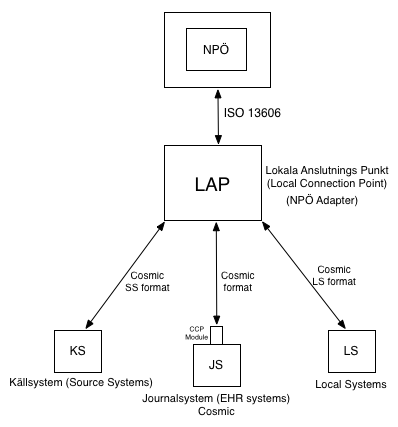
\includegraphics[width=0.32\textwidth]{Images/npoAdapt}
\end{figure}\

\subsection{Solutions}
There are two takes on the solution to interoperability that are generally accepted.  Since interoperability is essentially making sure that two or more systems can exchange information, the two most popular solutions are to either make sure that all systems are capable of using the same data formats (Syntactic) or there exists some way for the systems to automatically interpret the other data formats used that they do not support (Semantic).

Of course, each of these solutions comes with both advantages and disadvantages.  While semantic interoperability might be quicker and less work at first, it is not practical if the number of systems is going to be expanded because then the automation process must be updated every time that happens.  Additionally, implementing semantic interoperability only requires that you know the output of the system for the changes to be made while syntactic interoperability requires complete knowledge of the workings of the system as a whole for the changes to be made.  In return, syntactic interoperability is more work up front but does not require any of the existing systems to be updated when new systems are added.

\subsection{Prerequisites for interoperability on a national level}

To achieve European wide solutions for cross-border transfer of patient information certain requirements need to be fulfilled. There has to be an agreement on the definitions of data sets for both patient summaries and e-prescription, a legal framework for data transfer, a technical framework to connect the systems at each level and a working semantic \gls{interoperability}. \cite{epSOS1}

\subsection{Care plans}
[Emil and Sam: Explaining what it is.]

\newpage

\section{Technical Standards}
\label{sec:TechnicalStandards}

\subsection{What is a Technical Standard for Computer Software?}
A technical standard is a recognized and established requirement about software systems that establishes the ``way things should be done." They are responsible for everything from the uniformity of web browsers (although not all browsers strictly conform to the standard) to the ability for nearly any laptop to connect wirelessly to any access point. Such standards specify aspects of a program such as a common format for a file or data transfer that allow different developers to develop separate software programs while allowing for \gls{interoperability} between the different systems. Software standards are the foundation for the \gls{interoperability} of different software systems.

\subsection{The Creation of a Standard}
Typically for different parties (software development companies) to agree on a specific software standard they create a software standards organization that consist of members and representatives of the various software companies who contribute ideas and opinions about making a single, unified standard addressing the data \gls{interoperability} problem that needs to be addressed.

\subsubsection{Examples of Software Standards Organizations}

\begin{itemize}
\item World Wide Web Consortium (W3C) - Responsible for web standards such as HTML, HTTP, and XML 
\item Institute of Electrical and Electronics Engineers Standards Association (IEEE Standards Association) - Responsible for a wide range of standards for engineering such as the 802.11 standard
\item Internet Engineering Task Force (IETF) - Responsible for providing standards for new Internet related technology 
\end{itemize}

\subsection{Adherence to Standards}
Adherence to a particular software standard can be either mandatory required or voluntarily followed. For example, in the United States banking software must conform to security standards and regulations set forth by the Federal Deposit Insurance Corporation (FDIC). Any system that does not conform to these standards faces legal action by the federal government and as such is not allowed for use by U.S. banks. On the other end of the spectrum, the standards set forth by the W3C as to how a web browser should interpret and render various web pages is a completely voluntary standard and while most popular, modern browsers do conform in the most part to these standards there are many cases where some (if not all) do not completely achieve compliance. However, they face no legal retaliation for not complying with the W3C's standards as the standards are voluntarily adhered to and not legally mandated.

\subsection{Software Standards and EHR Software}
With the growing ubiquitousness of the Internet, computers, and modern technology as well as the geographic diversity of medical talent and information it is doubtless that someday a standard specifying the transmission, storage, and format of electronic healthcare records will be developed; the benefit of such a standard is too great to be ignored for long. Such a standard will require and large organization to oversee and develop as patent data is widely varied and medical breakthroughs are discovered daily requiring such a standard to be constantly updated and modified to stay relevant. 

\subsection{Ideal EHR Standard}
All medical institutions have different needs and demands  are often very significant; This makes it exceedingly difficult to create a "one-size fits all" \gls{EHR}. An ideal \gls{EHR} standard will follow the trend of historically successful interfaces, that is that it will closely replicate the old paper version. It would also store the records in a standardized format as this maximizes interoperability and data mobility but allow for the interfaces to the system to be customized to the specific institution. Customizing each \gls{EHR} for the specific institution does add overhead development and maintenance costs but maximizes the workflow productivity at each facility while maintaining interoperability. 

\subsection{The Alternative to a Future Standard For EHR Software}
The only other option for sharing healthcare records would be to have a unified software system doctors all over the world would use to view and modify patient records. However, such a solution is unrealistic as for one there are already too many \gls{EHR} software companies to reasonably plan for one, new company to globally take over the entire electronic healthcare record industry. Furthermore, with anti-trust laws as well as fair competition clauses in many countries (such as the United States and Sweden) a single organization would not be legally allowed to be the sole producer of \gls{EHR} software systems.



\newpage

\section{Adoption of future systems}
\label{sec:Future}

\subsection{Technical limitations}

\newglossaryentry{Simple Object Access Protocol}{name = {Simple Object Access Protocol}, description = {is a protocol specification for exchanging structured information in the implementation of Web Services in computer networks}}

\newacronym[\glsshortpluralkey = SOAPs, \glslongpluralkey = Simple Object Access Protocol]{SOAP}{SOAP}{\gls{Simple Object Access Protocol}}

\newglossaryentry{Hypertext Transfer Protocol}{name={Hypertext Transfer Protocol}, description={a networking protocol for distributed, collaborative, hypermedia information systems}}

\newacronym[\glsshortpluralkey=HTTPs ,\glslongpluralkey= Hypertext Transfer Protocol]{HTTP}{HTTP}{\gls{Hypertext Transfer Protocol}}

\newglossaryentry{Extensible Markup Language}{name={Extensible Markup Language}, description={a set of rules for encoding documents in machine-readable form}}

\newacronym[\glsshortpluralkey=XLMs ,\glslongpluralkey=Extensible Markup Languages]{XML}{XML}{\gls{Extensible Markup Language}}

The technical limitations for an \glspl{EHR} system are multi-faceted. Two separate approaches to a solution are outlined in the United States’ Department of Health and Human Services paper Health Information Technology: Initial Set of Standards, Implementation Specifications, and Certification Criteria for Electronic Health Record Technology. \cite{AMA} 

One solution is to use a \gls{SOAP} which is a specification for exchanging structures information. This setup relies on the \gls{XML}, a remote procedure call, and the \gls{HTTP}. This system creates several layers of specifications for layer formats. This solution is very dependent on multiple different systems, which creates a problem for dependency. If one of the needed layers for specification goes down or malfunctions than the system as a whole will not work. 

Additionally, because of the use of the \gls{XML} format, the \glspl{SOAP} protocol will be slower than other options. This might cause a scalability problem for a large system. Also when relying on \glspl{HTTP} as a transport protocol the roles of the interacting parties are fixed therefore only the client can use the services of the other. These limitations to the design may cause future problems implementing a \glspl{SOAP} style system on a large scale.



\subsection{Legal issues}

The new Swedish legislation provides new opportunities, but not obligations. \cite{RiR19}

\glspl{EHR} exist to promote patient safety, high quality health care and minimized cost. It is also supposed to be a source of information for the patient (ch 3, § 2). A patient journal must be kept for each patient and may not be common to several patients. The one writing in the journal is responsible for that part. All journal entries must be written in Swedish. \cite{PatientDataAct}
\\\\
The patient is not required to give his or her consent for the \gls{HCP} to act according to what the Patient Data Law dictates, except for an EHR to be shared from one caregiver to another, when gaining electronic access to records of another care unit or during unified journaling. Patients may refuse to be part of organized records (kvalitetsregister). To remove parts of a journal there has to be convincing reasons, the part being removed can't be necessary for future health care and there should be no public interest in keeping the information. Journal data may be blocked from unified journaling access but the information saying that data has been blocked and by who should still be available. A caregiver may have access to documented information only if he or she participates in the care of the patient or for other reasons need this information for their work in health care. The law also regulates periodical checking of the logs. The patient has rights to obtain certain parts of his or her medical journal and information on who has accessed it in the past.\cite{PatientDataAct}
\\\\
The Personal Data Privacy Act (1998:204) applies to the parts of the records that are managed automatically and stored in a structured fashion. The National Board of Health and Welfare has rights and obligations regarding apprehension of journals in the event of legal violations.\cite{PatientDataAct}
\\\\
According to the Swedish Patient Safety Act (2010:659), a caregiver must immediately inform a patient who has suffered a medical injury
about the injury, planned preventive measures, complaint and compensation
options and the patient councils activity. Information on the information provided shall be recorded in the patient record.\cite{PatientSafetyAct}
\\\\
If with regard to the purpose of ongoing health care is of considerable importance
that the data is not provided to the patient, then the caregiver is not allowed to
do so. Same thing applies if there is risk of violence or permanent damage to the
patient, should the information be disclosed. Also (unless enforced by law), a caregiver is not allowed to disclose details of health or personal conditions about a patient to outsiders.\cite{PatientSafetyAct}

\subsection{Organizational issues}
%[Emil and Erik: Current organizational issues that limit the adoption of interoperating systems.]
It is important to realize that in order to successfully implement a new system for \gls{EHR} sharing we need to have all the layers of the organization involved~\cite{Empirica} including all the different types of employees such as doctors and nurses etcetera. They must commit to the change of system in order for the switch to go well, since it changes the way they work and what responsibilities they have~\cite{Empirica}. In order to get all the different layers of the organization interested in the system it's important to involve them in the development of the system~\cite{Empirica}. Instead of having just the managers talking to the developers, all of the layers should be involved in the development stage of the system so that they feel like they have a say about the system that they will eventually use.
\\\\
When developing \gls{EHR} systems it is important to have clear objectives, ability to continuously revise changes and most importantly strong project leaders with the backing of the top level management and politics~\cite{Empirica}. This ties in to the previous topic of having all the layers of the organization involved in the development of the system. The employees might not be sure of exactly what they want so we need to make sure that when implementing a new feature or changing an existing one it is easy to make changes to the implementation in case of a misunderstanding between the developers and the employee who requested the feature.
\\\\

%Here are related items from the Empirica interview
%\begin{itemize}
%\item When it comes to \gls{interoperability}, technical issues and standard specifications are subordinated to legal and organizational %issues. The organizational issues include common understanding from people involved in the process and getting the commitment from %doctors and nurses. 
%\item Clear objectives and strong project leaders with the backing of the top level management and politics are very important factors of %success for \gls{EHR} projects. Continuous development and the ability to revise things are also crucial.
%\item It is important to reach all the layers of the health care organization to achieve change, to engage the different groups of doctors, %nurses, secretaries, technicians and not only have the software developers talk to the management section of the organization.
%\item Electronic systems are changing the way doctors work and what responsibilities they have.
%\end{itemize}

\newpage

\section{Results/ Discussion}
\label{sec:Results}

\subsection{Prerequisites for increased interoperability}

\subsection{Types of solutions and implications for the end user}

\subsection{EHR as a Standalone Application}
One possible interoperating system granting health personnel access to patient records from different hospitals would be a standalone application separated from existing EMR systems. Health care units would need to implement an interface towards the interoperating system to make their health records available. 

This raises a few concerns regarding the ownership of data, and who actually controls the data and keeps track of existing copies etc. The design of such a system could be either centralized with a data-cluster collecting patient information, or using a decentralized structure only accessing the patient information temporarily upon a specific query. By integrating the system into their previous EHR system the hospital would then give access to their health records. Then, whenever a user (from any hospital with this application installed) searches for information on a specific patient, the application would be able to search every hospital connected to the system. These searches could be narrowed to specific hospitals if, for example, a doctor had already run a search on a patient and wanted to find his/her information again, or knew which hospital that patient had been to. Essentially each hospital would have its own account, labeled as that hospitals name. Any other hospital could search its own database, or another hospitals database, or all databases.

A standalone system could be implemented either as a desktop application or in a web application. From a usability perspective a standalone application could cause a few usability issues. This doesn’t take advantage of the users knowledge of the legacy system as they have to learn a new user interface specific for the interoperating system. A workaround for this could be to allow individual hospitals to customize the end user interface to accommodate differences in user needs.

Another issue is that a standalone application forces the end user to multi-task between the legacy EHR system and the new interoperating application. This increases the complexity of the work environment as it doesn’t take advantage of human cognitive capabilities and adds a burden on the human memory.

A standalone system could be implemented with an interface for patients to access their Personal Health Records from their home computers. This would be a useful way for patients to obtain the various medical records that are shown to schools, employers, or whoever they may need to share medical information with. Additional features could also be implemented into the health records to extend it’s functionality with self-care and preliminary test before visiting a health care unit. This will also become helpful for certain security issues, as will be discussed in the next section.

\subsubsection{Security}
This standalone application does cause a few security concerns. Hospitals would have to be careful about which data they allow the application to access. If a hospital is storing sensitive data about a patient that cannot be shared without that patients consent, a few problems occur. A simple, though impractical, solution would be to have the hospital create a separate database for sensitive information. Again, this simply is not practical. The extra upkeep would be costly and searching two databases each time a doctor needs information on one patient is time consuming. Instead, the data on each patient can be labeled as sensitive. The application would then know not to share this data, unless permission is given. But how should permission to view sensitive data be given? There are two viable options here. Either have the patient create a password that is only shared with those who are allowed to view the data, or have an administrative control deciding who can and cannot view the data. The first option is far easier to use and can allow permission to be given out quickly. The main problem with passwords is that they are not very secure. The password could be stolen, accidentally released, or guessed by another. Once a doctor knows the password that doctor can share it with anyone, regardless of what the patient says. While this is an easy solution, it is not very secure. Administrative control, on the other hand, is secure. In this scenario, only the account that uploaded the sensitive data can view it. Then, that account must give permission to another account to view the data. This requires a few things. First, an individual account must be created. Anytime a search on that patient is run, sensitive data will be hidden unless the searcher requests permission from the account owner. The owner would then be free to give or refuse permission. This would be a more time consuming process than the first option, but quite a bit more secure. These individual accounts do not need to be able to modify any medical records, only give permission to other accounts to access the sensitive data regarding a certain patient.

\subsubsection{Interoperability}
A common problem our solutions run into is the degree to which hospital databases can vary. In this scenario, one application needs to be able to search many different databases. None of these databases necessarily work in the same way. Trying to make an application that could properly read every part of each database would be impractical. This can be solved if the application only retrieves entire sections listed under a specific patient. The application would not be able to retrieve exact details about a patient. Instead it would find a file regarding that patient and return it to the user. This may result in larger amounts of information being retrieved than the user wanted or needed, but this is hardly a concern as long as they get the actual data.
Additional problems in this area can be resolved by also allowing a message function. This would be a fallback if the application is completely unable to work with a certain file or database system. One hospital would be able to send a message to another, requesting a file on a patient. This would be a much slower process, but at least it still gets the work done.

\subsubsection{Feasibility}
The biggest difficulty with creating this standalone application is ensuring that it can interact with various different database systems. Fortunately there are a lot of standards and regulations regarding database systems and medical records. These should help to limit the variations in systems and are discussed in greater detail in the section 6. 

\subsection{EHR integrated into existing EMR systems}

\subsubsection{Interoperability}
To make a system like this work within all the existing EHR systems it needs a really good 	interoperability. The existing EHR systems are structured in very different ways. The data is both written and stored in different ways.
There are however similar industries that have the same issue but have solutions to work around this problem to make it more transparent way. Within the European Union there is a border management system where each EU member state perform their operational tasks independently based on a regulatory framework managed by the European Commision. By using a set framework and a set standard all the different system can be merged in one format in a central unit. This framework should include a certain semantics so that the data can be transferred in a smooth way between the systems. The systems layout doesn’t need to change as long as what they send to the central unit follows the set standard.

\subsubsection{Technical}
In a system this big there is a risk that a lot of data will be handles back and forth. There are regulations on where data is stored and that a patient can request it's deletion. To be able to follow these regulations a central database could be used. Each EHR system stores the data they have in their system but also stores the same information in the central database. That way the central database keeps a complete record for each patient. The data however never get copied from the central database. When looking at a patients record in any of the EHR systems it reads from the central server. With a system set up like this data stored will only be stored at two places, in the EHR system where it was created and in the central database. This makes a deletion of data easy.
The system also has to be secure, no unauthorized users should be able to access data. As the users are using the old EHR systems, where they have authentication to able to access information, all that is needed is that every EHR system fulfil a required standard for security. The whole system can also be kept in a intranet to avoid intrusion even further.

\subsubsection{Feasability}
One of the problems with implementing a system like this is to get all the systems to unit and accept a set standard to be used. Some of the systems has to change more then others.
Having a large central database for all EHR data (Sweden) could be considered hard to manage but according to Johan Thorvid it should be feasible.

\subsubsection{Usability implications}
This integrated solution is supposed to have as small implication as possible for the users. There might be some small changes as the systems that they are currently using may have to change a bit to be able to meet the standards that are going to be used. As the semantics has to match some of the users may have to change how they write. However with a integrated solution the user can do all the work in the system they are currently using. Most of the old systems will however still be intact and the users can use the old knowledge and experience when navigating.

\newpage

\section{Conclusions}
\label{sec:Conclusions}
\subsection{Recommended Development Methodologies}
The interviews with administrative personal and technicians were focused on what they thought would be required to create interoperability between \glspl{EHR} rather than what they would want in such a system. 

One of the most important things learned from these interviews was that the development of an interoperable system would be very complex. It is hard to define a definite end in such a big development process and the process should be considered on-going where focus lie on completing sub-goals rather than only shooting for the final goal. In other words the work should be approached with a type of agile development. 

Agile development is an iterative and incremental development process where the work is done in small steps and every step is evaluated. The small steps could be subparts of the final system. Starting off with a smaller part of the system, ensuring that this part works and then move on by adding more features or go on to the next part of system might be more successful than trying to complete the whole system at once. However, this could be very time consuming and is not an option if there is a short amount of time to complete the system. It is therefore important to consider the amount of time and resources that can be spent on the project against the size of the iterative steps in the agile development.


Another important aspect that came up during the interviews was the involvement of the end-user in the development process. The end-user in an interoperable system between \glspl{EHR} is the users of the \glspl{EHR} such physicians, nurses etc. If the development of the interoperable system can not be done only in the back-end, meaning that the end-user's systems will be affected, their opinions will be of importance. In this case the change in the systems might be made in a way that does not affect the end-users negatively if their opinions are taken into consideration in the development. Even if there is no need for noticeable changes their opinions can still be of importance when it comes to what kind of patient information that is most important to share in the interoperable system if it is unmanageable to share all information. 

The involvement of end-users can be included in the agile development by letting them take part in the evaluation of the sub-parts where their opinions matter. 

During the interviews the issue regarding security came up as an important factor to consider in an interoperable system. It is always important to handle the security with great care when it comes to patient information, but the security issues might be a lot greater when dealing with a system of bigger size such as when multiple \glspl{EHR} is interoperating. One example of a feature that might need improvement is the access control of patient information due to the fact that an interoperable system will increase the amount reachable information. Ordinary methods for checking access control such as going through logs might be inefficient and costly and new methods might be needed.


\newpage
\printglossaries
\newpage

\begin{appendix}
\end{appendix}



\bibliographystyle{unsrt} 
\bibliography{ourBib} 

\end{document} 
